% Inbuilt themes in beamer
\documentclass{beamer}
\usepackage{graphicx}
\usepackage{changepage}
\usepackage[backend=biber, style=ieee]{biblatex}
\usepackage{subscript}
\usepackage{gensymb}
\addbibresource{bibliography.bib}


% Theme choice:
\usetheme{Frankfurt}

% Title page details:
\title{Decentralizing Agriculture}
\subtitle{A shift in the industrial paradigm of food production}
\author{Marco Zolla Salazar}
\date{\today}
\logo{\large \LaTeX{}}


\begin{document}

% Title page frame
\begin{frame}
    \titlepage
\end{frame}

% Remove logo from the next slides
\logo{}


% Outline frame
\begin{frame}{Outline}
    \tableofcontents
\end{frame}


\section{The many problems of industrial agriculture}

\begin{frame}{Land use and biodiversity loss}
    \begin{itemize}
        \item Cropping and animal husbandry cover over one third of the terrestrial land surface; agriculture drives roughly 90\% of global deforestation \cite[XVI]{IPBES2019GlobalAssessment}, \cite[4]{FAO2025StateFoodAgri}. \vspace{6mm}
        \item More than 90\% of biodiversity impacts from land-use change are attributable to agriculture --- crops alone account for 72\% \cite{cabernard2024biodiversity}. \vspace{6mm}
        \item A 27-year study found a 76\% decline in flying insect biomass; European farmland birds fell 57\% over 37 years \cite{hallmann2017insect}, \cite{rigal2023farmlandbirds}.
    \end{itemize}
\end{frame}

\begin{frame}{Soil degradation}
    \begin{itemize}
        \item Conventional tillage erodes soil one to two orders of magnitude faster than it forms --- ``fundamentally unsustainable over civilizational timescales'' \cite{montgomery2007soil}. \vspace{6mm}
        \item Cropland soils have lost 20--60\% of their pre-cultivation organic carbon \cite[TS.4]{ipcc2019srccl}. \vspace{6mm}
        \item A meta-analysis of 25,000+ studies confirms 16--25\% SOC loss following conversion of grassland or forest to cropland \cite{beillouin2023soc}.
    \end{itemize}
\end{frame}

\begin{frame}{Chemical inputs: pesticides and fertilizers}
    \begin{itemize}
        \item 64\% of global agricultural land is at risk of pesticide pollution; 31\% at high risk \cite[206]{Tang2021}. \vspace{6mm}
        \item Fertilizer runoff has driven the spread of coastal dead zones to over 500 documented systems worldwide \cite{breitburg2018oxygen}. \vspace{6mm}
        \item Agricultural N\textsubscript{2}O emissions have grown 40\% since 1980, exceeding all CMIP6 emission scenarios \cite[Section~4.2.1]{Tian2024}.
    \end{itemize}
\end{frame}

\begin{frame}{Monoculture and structural lock-in}
    \begin{itemize}
        \item Diversified rice plantings suffered 94\% less rice blast and yielded 89\% more per hill than monoculture \cite[718--721]{zhu2000genetic}. \vspace{6mm}
        \item Global banana production hangs on a single cultivar (Cavendish); its predecessor was wiped out by Fusarium wilt --- and is now under threat from a new strain \cite[2147--2150]{kema2021vulnerability}. \vspace{6mm}
        \item Four firms control 56\% of the global seed market and 61\% of pesticides --- agronomic uniformity is a structural outcome of input-market concentration \cite{etcgroup2025agribusiness}, \cite{howard2009consolidation}.
    \end{itemize}
\end{frame}

\begin{frame}{Freshwater depletion and greenhouse gas emissions}
    \begin{itemize}
        \item Agriculture accounts for 70--85\% of global freshwater withdrawals \cite{puy2025irrigation}. \vspace{6mm}
        \item Five crops drove most of the 22\% rise in global groundwater depletion between 2000 and 2010 --- much of it from non-renewable aquifers \cite{dalin2017groundwater}. \vspace{6mm}
        \item The agrifood system emits $\sim$30\% of all anthropogenic GHGs (16.2~Gt~CO\textsubscript{2}eq); on a business-as-usual path, food alone could exhaust the 1.5\degree C carbon budget \cite{fao2024ghg}, \cite{clark2020foodclimate}.
    \end{itemize}
\end{frame}

\begin{frame}{Supply-chain externalities: transport, storage, food waste}
    \begin{itemize}
        \item 25--30\% of food produced is lost or wasted; food loss and waste alone account for 8--10\% of anthropogenic GHGs \cite[Section~5.5.2.5]{ipcc2019srccl}. \vspace{6mm}
        \item Cold-chain refrigeration emits $\sim$10\% of all agrifood GHGs and has more than doubled since 2000 \cite[Section~3]{flammini2024coldchain}. \vspace{6mm}
        \item Food waste is responsible for an estimated 58\% of US landfill methane, with 61\% escaping uncaptured \cite[Table~3]{epa2023methane}.
    \end{itemize}
\end{frame}

\begin{frame}{Concentration and dependency at every level}
    \begin{itemize}
        \item \textbf{Country level} --- 7 countries plus the EU produce 88\% of world wheat exports; most nations depend on a handful of suppliers \cite[16]{usda2025grain}. \vspace{4mm}
        \item \textbf{Corporate level} --- four firms dominate the global seed (56\%), pesticide (61\%), and machinery (43\%) markets \cite{etcgroup2025agribusiness}. \vspace{4mm}
        \item \textbf{Community level} --- 0.1\% of farms operate over half of all agricultural land; the 85\% of farms under 2~ha hold just 9\% \cite[Chapter~3]{fao2025sofa}.
    \end{itemize}
\end{frame}

\begin{frame}{Suppression of dietary diversity and nutritional decline}
    \begin{itemize}
        \item Industrial systems funnel commodity outputs into ultra-processed foods, linked to higher cardiovascular mortality, type-2 diabetes, and obesity (umbrella review, $\sim$10M participants) \cite[Figures~2--3]{lane2024upf}. \vspace{6mm}
        \item Wheat zinc, copper, and magnesium concentrations declined 20--49\% after the introduction of high-yield cultivars in the 1960s \cite[Tables~2,~4]{fan2008nutrient}. \vspace{6mm}
        \item Nutritional decline tracks the narrowing of crop genetic diversity that monoculture demands \cite{monteiro2025upf}.
    \end{itemize}
\end{frame}


\section{Research methodology}

\begin{frame}{An iterative, source-grounded verification pipeline}
    Three custom slash commands form a single research pipeline:
    \begin{itemize}
        \item \texttt{/verify-paper} --- paper-wide audit; one subagent per section dispatched in parallel; produces a master corrections table. \vspace{4mm}
        \item \texttt{/verify-section} --- interactive, claim-by-claim verification of citations, narrative, and structure for one section. \vspace{4mm}
        \item \texttt{/expand-section} --- gap-filling pass; identifies missing evidence and surfaces cross-section relevance. \vspace{4mm}
        \item All findings persist in \texttt{sources/corrections.md} as stable IDed items, working across multiple sessions.
    \end{itemize}
\end{frame}

\begin{frame}{Per-citation verification protocol}
    \textbf{One subagent per source file}, reading both:
    \begin{itemize}
        \item OCR text --- statistics, quotes, exact wording.
        \item Original PDF --- figures, tables, layout.
    \end{itemize}
    \vspace{2mm}
    \textbf{Each claim is checked for:}
    \begin{itemize}
        \item Factual and temporal accuracy
        \item Primary vs.\ secondary attribution
        \item Scope and caveats preservation
        \item Disconfirming evidence in the surrounding text
        \item Bibliography metadata (author, year, DOI)
    \end{itemize}
    \vspace{2mm}
    The orchestrator independently spot-checks every non-OK verdict before any edit; pinpoint locators (\texttt{\textbackslash cite[Section~X]\{key\}}) are required on every modified citation.
\end{frame}

\begin{frame}{Standing principles}
    \begin{itemize}
        \item \textbf{No sycophancy} --- ideas are evaluated against the thesis before agreement; corrections are preferred to retractions. \vspace{6mm}
        \item \textbf{Primary sources only} --- every secondary citation is flagged to the user, never filtered out by the assistant. \vspace{6mm}
        \item \textbf{Reproducibility} --- every claim must be traceable to a source on disk; no verification from model memory. \vspace{6mm}
        \item \textbf{Failure mode avoided} --- confident citation of things the source does not actually say.
    \end{itemize}
\end{frame}


\section{Background}

\begin{frame}{Case study: The Netherlands}
    \begin{itemize}
        \item ``Dutch greenhouses aren't your run-of-the-mill structures - they're technological marvels.'' \cite{hbs2024} \vspace{10mm}
        \item The Netherlands, despite its small land area, is the second-largest agricultural exporter in the world by value \cite{ITA2026_Netherlands_Agriculture}
    \end{itemize}
\end{frame}

\section{Proposed solution}

\begin{frame}{Objectives}
    \begin{itemize}
        \item Agriculture decentralization \vspace{10mm}
        %Local production -> local consumption
        %Smaller production batches -> less waste and pollution
        %More diverse produce -> more resilient food chain
        \item Optimize production efficiency \vspace{10mm}
        \item Create a scalable, automatic and widely available solution \vspace{10mm}
    \end{itemize}
\end{frame}

\begin{frame}{Architecture overview}
    \begin{adjustwidth}{-2em}{-2em}
    \centering
    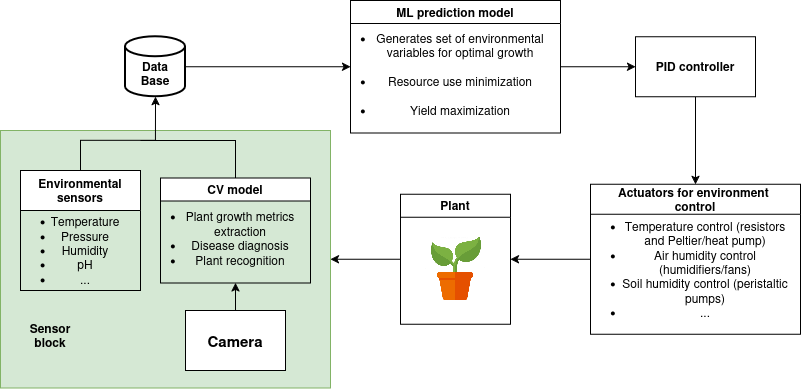
\includegraphics[width=1.1\textwidth, keepaspectratio]{img/architecture_overview.png}
    \end{adjustwidth}
\end{frame}

\begin{frame}{Optimization through collaboration}
    \begin{itemize}
        \item Open source hardware, software, models and data\vspace{10mm}
        %Privacy concern solved my edgeAI computer vision model
        \item Guides for personal and commercial use\vspace{10mm}
        \item Seed sharing communities and markets
    \end{itemize}
\end{frame}

\section{References}
\begin{frame}[allowframebreaks]{Bibliography}
\printbibliography[heading=none]
\end{frame}

\end{document}
